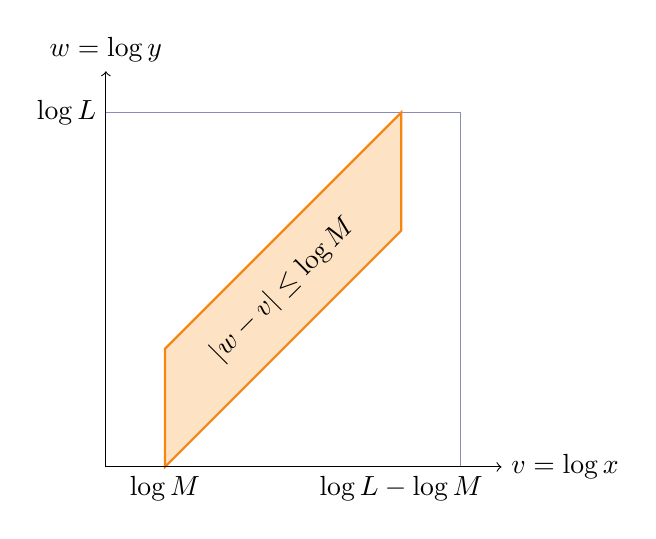
\begin{tikzpicture}[scale=.75]
\draw[MidnightBlue!50] (0,0) rectangle (6,6);
\fill[BurntOrange!20] (1,0)--(1,2)--(5,6)--(5,4)--cycle;
\draw[BurntOrange,thick] (1,0)--(1,2)--(5,6)--(5,4)--cycle;
\draw[->] (0,0)--(6.7,0) node[right] {$v=\log x$};
\draw[->] (0,0)--(0,6.7) node[above] {$w=\log y$};
\node[below] at (1,0) {$\log M$};
\node[below] at (5,0) {$\log L-\log M$};
\node[left] at (0,6) {$\log L$};
\node[rotate=45] at (3,3) {$|w-v|\le\log M$};
\end{tikzpicture}
